\documentclass[tikz,border=10pt]{standalone}
\begin{document}
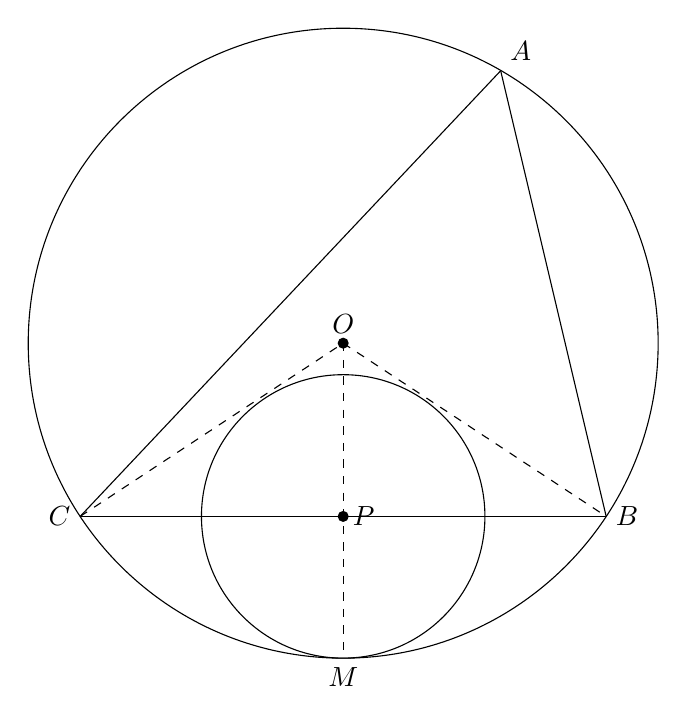
\begin{tikzpicture}
    \coordinate (O) at (0, 0);
    \coordinate (M) at (0, -4);
    \coordinate (P) at (0, -2.2);
    \coordinate (B) at (3.34, -2.2);
    \coordinate (C) at (-3.34, -2.2);
    \coordinate (A) at (2, 3.46);

    \draw (O) circle (4);
    \draw[dashed] (C) -- (O);
    \draw[dashed] (O) -- (B);
    \draw[dashed] (O) -- (M);
    \draw (P) circle (1.8);
    \draw (A) -- (B);
    \draw (A) -- (C);
    \draw (C) -- (B);
    
    \fill (O) circle (2pt);
    \fill (P) circle (2pt);
    
    \node[above right] at (A) {$A$};
    \node[right] at (B) {$B$};
    \node[left] at (C) {$C$};
    \node[above] at (O) {$O$};
    \node[right] at (P) {$P$};
    \node[below] at (M) {$M$};
\end{tikzpicture}
\end{document}
